\subsection[]{Mengenlehre}
\begin{definition}
Sei $M$ eine beliebige Menge. Die \textcolor{orange}{Potenzmenge von $M$} ist die Menge aller Teilmengen von $M$. Wir schreiben
\begin{center}
    \textcolor{orange}{$\mathcal{P}(M) \coloneqq \{X : X \subset M\}$}
\end{center}
Insbesondere gilt stets $\emptyset \in \mathcal{P}(M)$.
\end{definition}
\begin{definition}
Seien $M,N$ Mengen. Das kartesische Produkt von $M$ und $N$ ist die Menge
\begin{center}
    \textcolor{orange}{$M \times N = \{(m,n) : m \in M, n \in N\}$}
\end{center}
\end{definition}
\begin{definition}
Ist $m \in M$ und $n \in N$, so heißt $(m,n) \in M \times N$ \textcolor{orange}{geordnetes Paar} und hat die Eigenschaft: 
\begin{center}
   $(m,n) = (m',n')$ \textcolor{red}{genau dann, wenn} $m = m'$ und $n = n'$ 
\end{center}
\end{definition}
\newpage
\begin{remark}
Wahrheitstafel: 
\begin{center}
    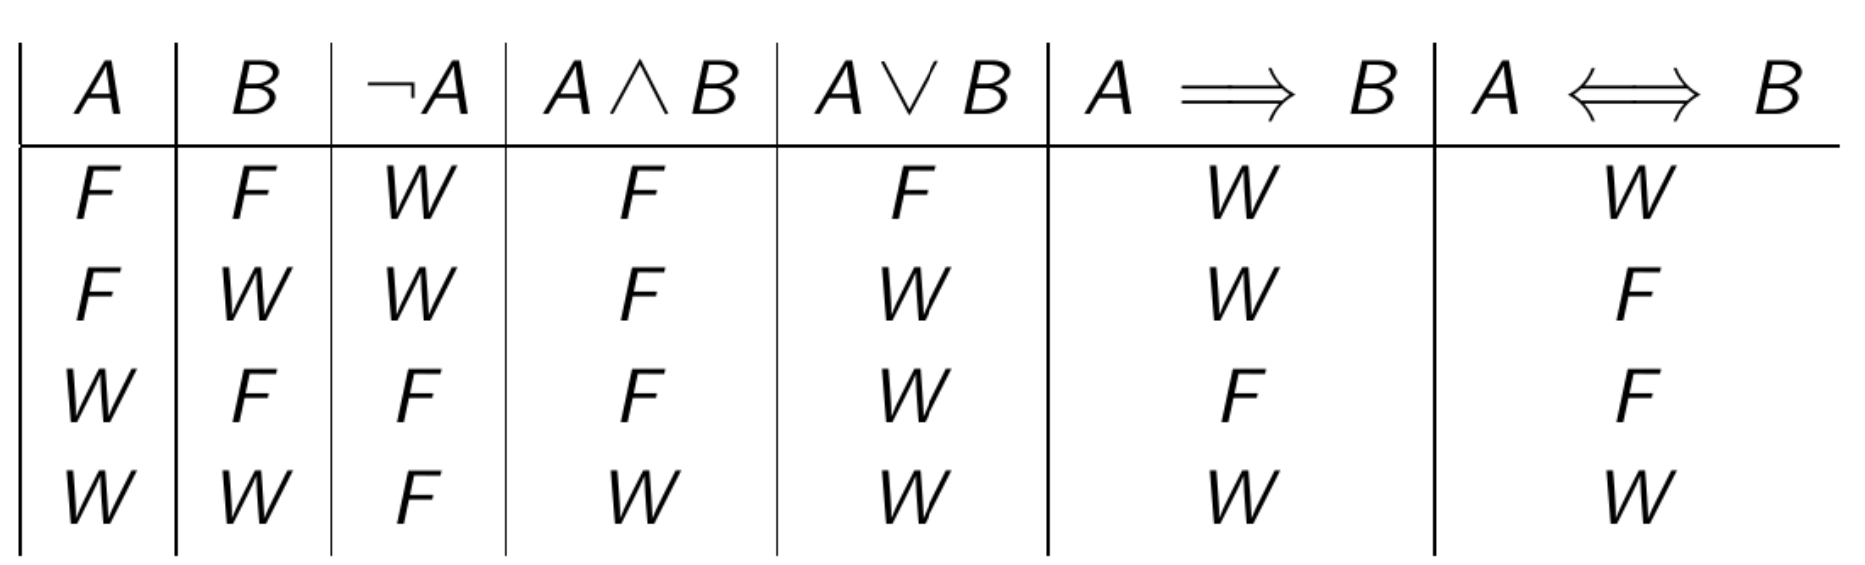
\includegraphics[width = 8 cm]{Wahrheitstafel.png}
\end{center}
\end{remark}
\subsection[]{Beweise}
\begin{definition}
Direkter Beweis:
\begin{center}
     Voraussetzung(en) $\Rightarrow$ Behauptung
\end{center}
\end{definition}
\begin{definition}
Indirekter Beweis:
\begin{center}
    $(A(x) \Rightarrow B(x)) \Leftrightarrow (\neg B(x) \Rightarrow \neg A(x))$
\end{center}
\end{definition}
\begin{definition}
Widerspruchsbeweis:\\
Wir möchten die Wahrheit der Aussage A beweisen.\\
Dafür:\\
1) wir nehmen an, dass $\neg$A gilt\\
2) wir finden einen Widerspruch (mit Annahmen, logischen Argumenten,...)\\
3) daraus folgt: A gilt.
\end{definition}
\begin{definition}
Das Prinzip der vollständigen Induktion:\\
Es sei eine Aussage $A$ zu beweisen, die von der natürlichen Zahl $n$ abhängt, $A(n)$.\\
Angenommen:\\
1) Die Aussage A(1) gilt (Induktionsanfang);\\
2) Für alle natürlichen Zahlen $m$:
\begin{center}
    falls $A(m)$ (Induktionsvoraussetzung) gilt, so gilt $A(m+1)$ (Induktionsschritt). 
\end{center}
Dann gilt $A(n)$ für alle natürlichen Zahlen.
\end{definition}
\subsection[]{Abbildungen, Kardinalität von Mengen und Relationen}
\begin{definition}
Seien $A,B$ Mengen. Eine Abbildung $\alpha$ von $A$ nach $B$ ist eine Relation des kartesischen Produkts $A \times B$, d.h $\alpha \subset A \times B$ mit der Eigenschaft
\begin{center}
    \textcolor{blue}{zu jedem Element $a \in A$ gibt es genau ein Element $b \in B$ derart, dass das Paar $(a,b)$ in $\alpha$ liegt. Es ist $b = \alpha(a)$.}
\end{center}
\end{definition}
\begin{definition}
Ist $a \in A$, so heißt $b=\alpha(a)$ das \textcolor{orange}{Bild von $a$} unter $\alpha$.
\end{definition}
\begin{definition}
Die Menge Bild$\alpha \coloneqq \{ b \in B : \exists a \in A : b = \alpha(a)\} = \{ \alpha(a) : a \in A\}$ heißt das \textcolor{orange}{Bild von $\alpha$}.
\end{definition}
\begin{definition}
Eine Abbildung $\alpha:A \rightarrow B$ heißt \textcolor{orange}{injektiv}, falls aus $\alpha(a) = \alpha(a')$ folgt stets $a = a'$.
\end{definition}
\begin{definition}
Eine Abbildung $\alpha:A \rightarrow B$ heißt \textcolor{orange}{surjektiv (auf B)}, falls Bild$\alpha = B$
\end{definition}
\begin{definition}
Eine Abbildung $\alpha:A \rightarrow B$ ist \textcolor{orange}{eine Bijektion von $A$ auf $B$}, falls $\alpha$ injektiv und surjektiv ist.
\end{definition}
\begin{definition}
Ist $N \subset B$, so definiert man die \textcolor{orange}{Urbildmenge} $\alpha^{-1}(N) \subset A$ durch 
\begin{center}
    $\alpha(N) =  \{a \in A : \alpha(a) \in N\}$
\end{center}
\end{definition}
\begin{definition}
Zwei Mengen $A,B$ heißen gleichmächtig ($A$ und $B$ haben die gleich Kardinalität) falls es eine Bijektion 
\begin{center}
    $f : A \rightarrow B$
\end{center}
gibt.
\end{definition}
\begin{definition}
\begin{enumerate}
    \item Die Menge $A$ heißt endlich, falls $A = \emptyset$, oder es gibt $n \in \mathbb{N}$, und eine Bijektion $f : \{1,2,...,n\} \rightarrow A$.
    \item In diesem Fall sagen wir, dass die Kardinalität von $A$, $n$ ist, und wir schreiben $\#(A) = |A| = n$.
\end{enumerate}
\end{definition}
\begin{definition}
Sei $A$ eine Menge mit $|A| = |\mathbb{N}|$, so heißt $A$ abzählbar unendlich.
\end{definition}
\begin{definition}
Eine Relation $R$ auf die Menge $M$ heißt
\begin{enumerate}
    \item \textcolor{red}{reflexiv}: falls $xRx$ gilt für jedes $x \in X$;
    \item \textcolor{red}{symmetrisch}: falls $xRy$ genau dann wenn $yRx$, für alle $x,y \in X$;
    \item \textcolor{red}{transitiv}: falls $xRz$ aus $xRy$ und $yRz$ folgt, für $x,y,z \in \mathbb{X}$.
\end{enumerate}
\end{definition}
\begin{definition}
Sei $X$ eine Menge, und ~ heißt \textcolor{orange}{Äquivalenzrelation} falls sie \textcolor{orange}{reflexiv}, \textcolor{orange}{symmetrisch} und \textcolor{orange}{transitiv} ist, d.h.
\begin{enumerate}
    \item für alle $x \in X$ gilt: $x \sim x$,
    \item für alle $x,y \in X$ gilt: $x \sim y \Leftrightarrow y \sim x$,
    \item für alle $x,y,z \in X$ gilt: aus $x \sim y$ und $y \sim z$ folgt $x \sim z$.
\end{enumerate}
\end{definition}
\begin{definition}
Sei $\sim$ eine Äquivalenzrelation auf die Menge $X$. Dann heißen, für $a \in X$, die Mengen
\begin{center}
$[a] \coloneqq \{x \in X : x \sim a\} =: [a]_\sim$
\end{center}
\textcolor{orange}{Äquivalenzklassen}(der Äquivalenzrelation $\sim$ ).
\end{definition}
\begin{definition}
Sei $X$ eine nicht leere Menge und $P \subset \mathcal{X}$. Dann heißt $P$ eine Partition falls:
\begin{enumerate}
    \item Für alle $A \in P$ gilt $A \neq \emptyset$,
    \item Für alle $A,B \in P$ gilt entweder $A=B$ oder $A \cap B = \emptyset$,
    \item Für alle $x \in X$ existiert $A \in P$ so, dass $x \in A$.
\end{enumerate}
\end{definition}
\begin{corollary}
Sei $X$ eine nicht leere Menge und $\sim$ eine Äquivalenzrelation auf $X$. Dann ist die Menge aller Äquivalenzklassen von $\sim$, nämlich $X/\sim$ eine Partition von $X$. 
\end{corollary}
